\documentclass[12pt]{article}
\usepackage{amsmath,amssymb,amsthm}
\usepackage[english]{babel}
\usepackage[utf8]{inputenc}
\usepackage{fancyhdr}
\usepackage{changepage} 

\usepackage{hyperref}

% for line spacing
\usepackage{setspace}

% for absolute value
\usepackage{commath}

% for numbering
\usepackage{enumerate}

% for image placing
\usepackage{float}

% paper size and margins
\usepackage[letterpaper, left=20mm, right=20mm, top=25mm, bottom = 25mm, headsep=.15in]{geometry}

% for code snippet
\usepackage{listings}

% for curly brace
\usepackage{amsmath}

% for input images
\usepackage{graphicx}
\graphicspath{ {./} }
\usepackage{subfig}

% for printing pseudocode
\usepackage[boxed]{algorithm}
\usepackage[noend]{algpseudocode}

% for tables
\usepackage{tabularx}

\makeatletter
\def\BState{\State\hskip-\ALG@thistlm}
\makeatother

% for circled numbers
\usepackage{tikz}
\newcommand*\circled[1]{\tikz[baseline=(char.base)]{
            \node[shape=circle,draw,inner sep=1pt] (char) {#1};}}

% double line space
\renewcommand{\baselinestretch}{2.0}

% header, footer and page number
\pagestyle{fancy}
\fancyhf{}
\rhead{Tiankai Jiang \quad 20834939}
\lhead{ECE657A \quad Assignment 3}
\fancyfoot[C]{\thepage}

\setlength{\headheight}{15pt}
\lstset{language=Python}
\begin{document}
\noindent
{\LARGE The source code is at the end of this document}
\section{Classification: Feature Extraction + Classical Methods}
\subsection{Explanation of Design and Implementation Choices of your Model}
The models I used on Kaggle are XGBoost, SVM, Random Forest and Hist Gradient Boosting. Below is the procedure to show why I chose them.

Dataset was given with labels, so naturally supervised learning methods were considered. There are 784 dimensions in the dataset, therefore, PCA should be applied on it to extract the main features and to decrease the dimension. First I used standard scalar to centralize data and then drew the scree plot with top 100 principle components.
\begin{figure}[H]
\begin{center}
    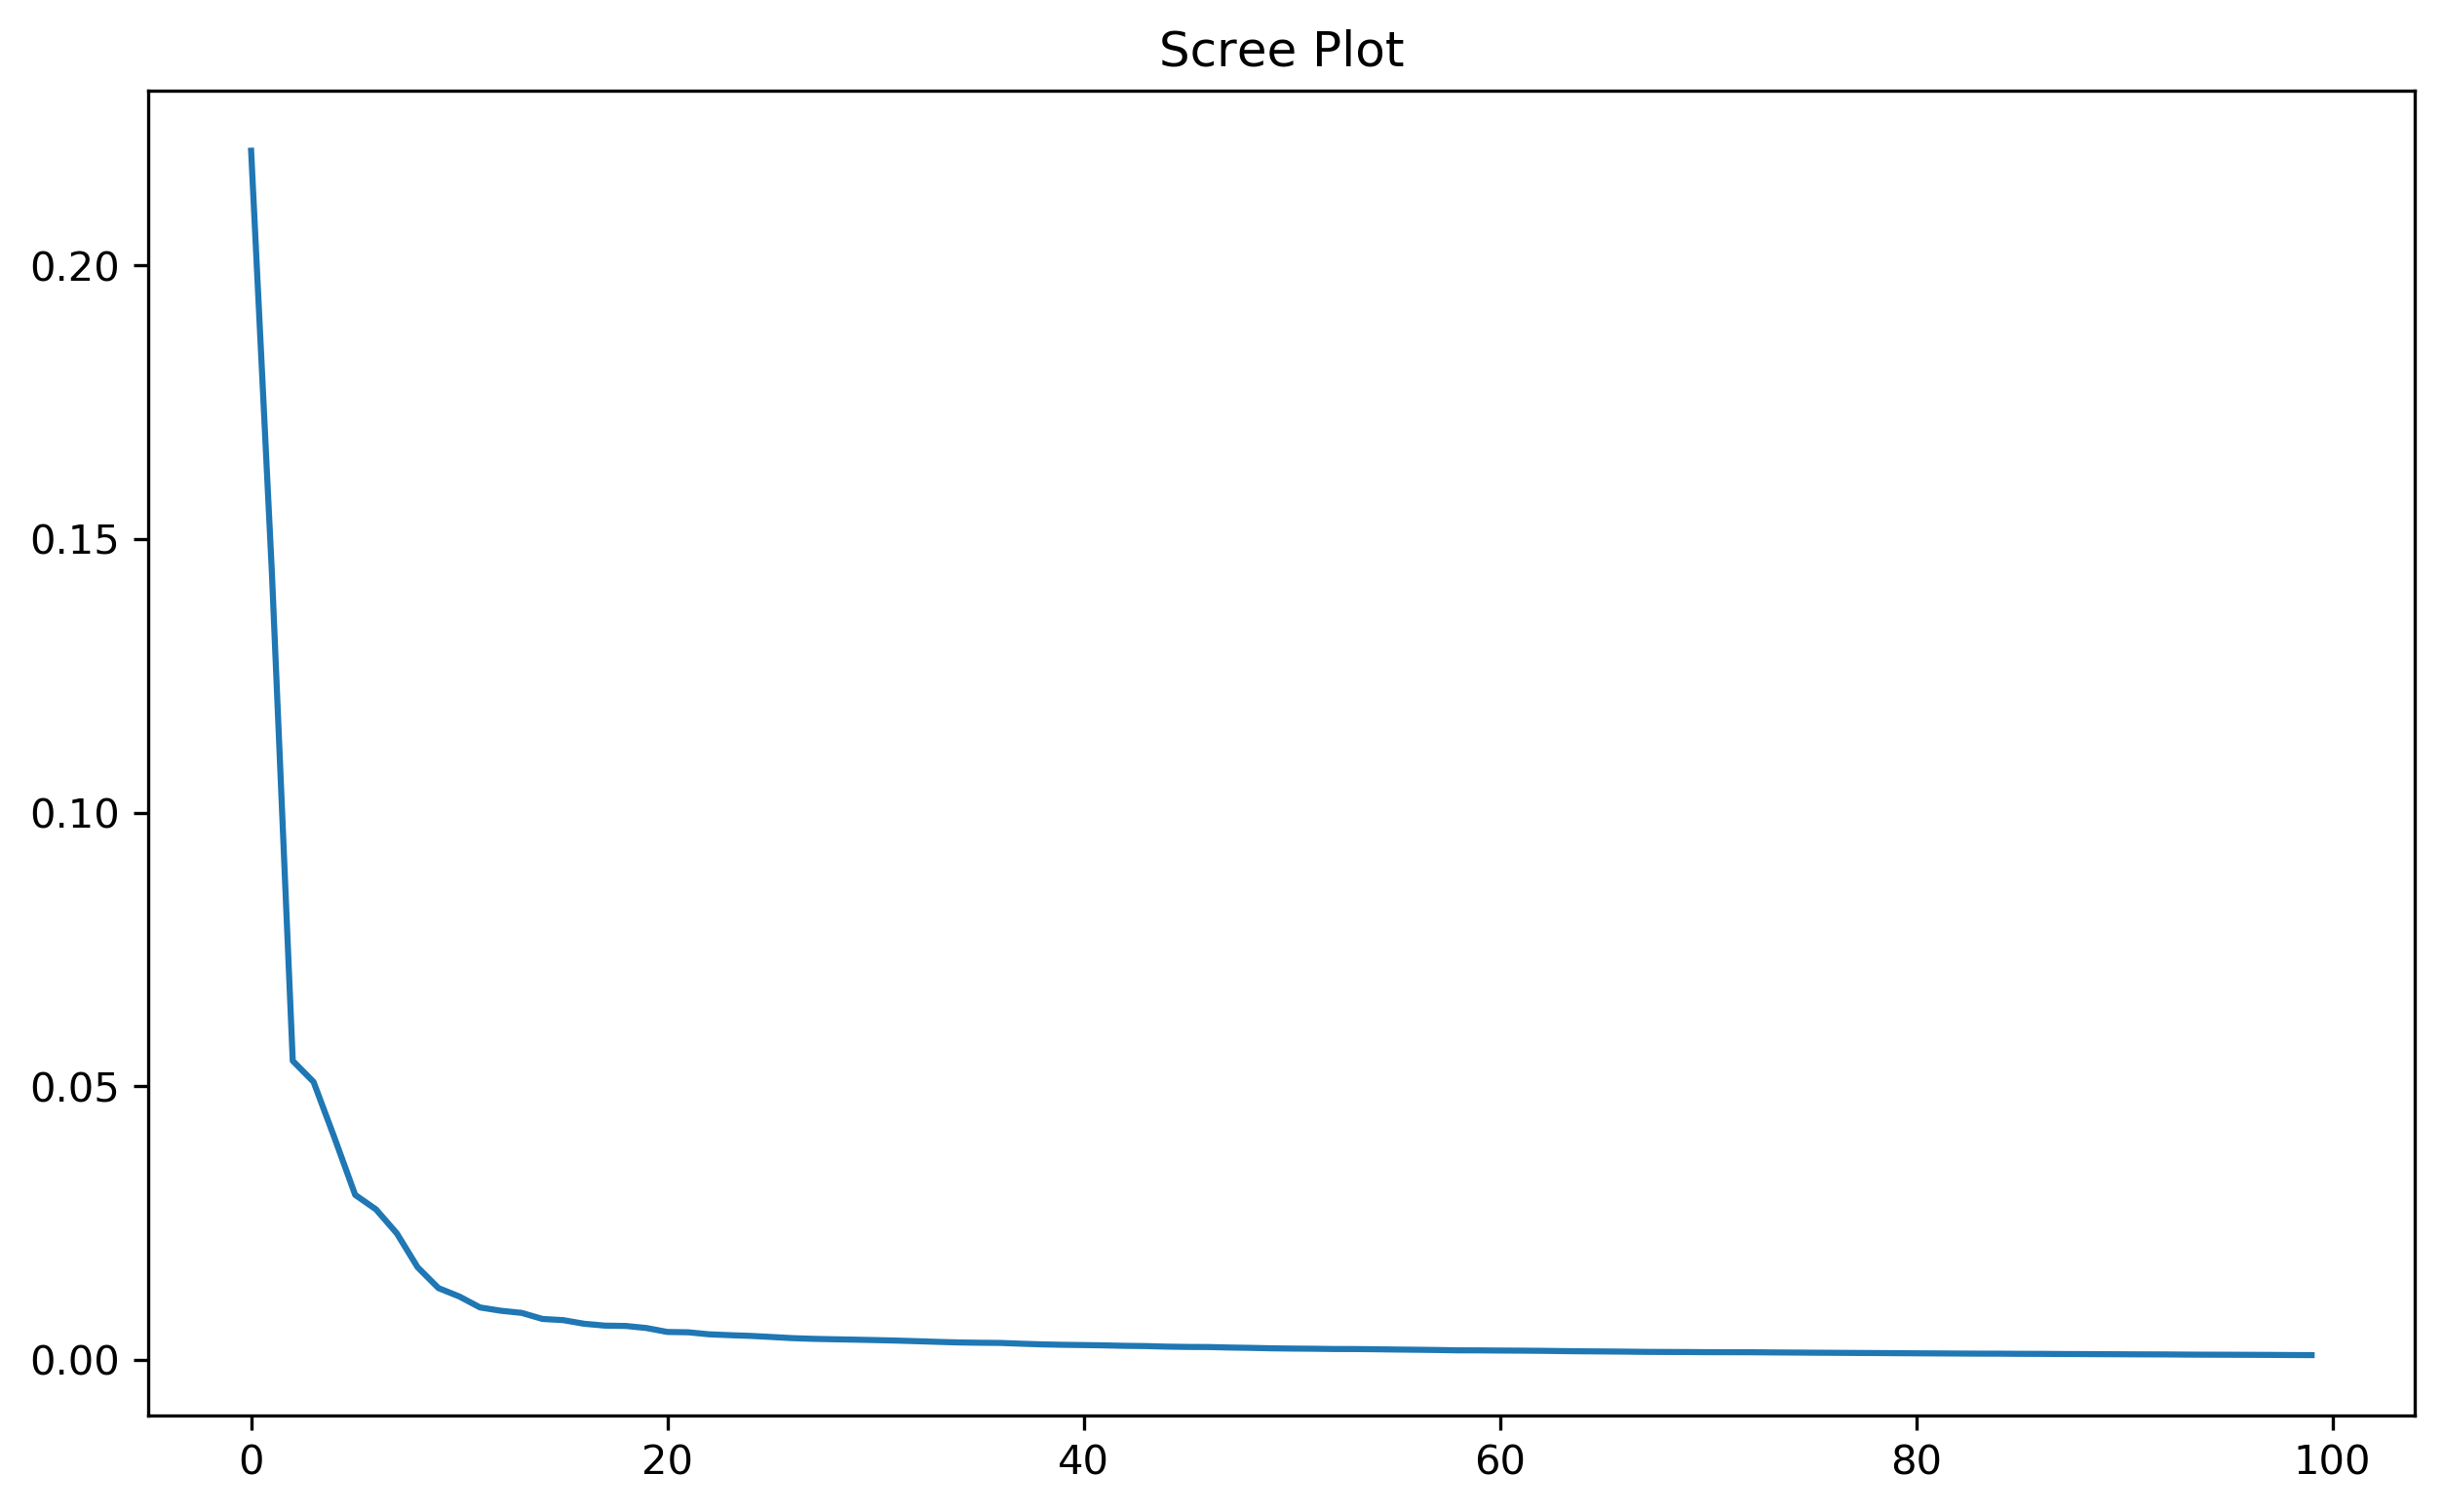
\includegraphics[width=0.7\textwidth]{./plots/ScreePlot.png}
\end{center}
\end{figure}
More than 99 percent of variance can be explained by the top 20 principle components. I took n\_components = 30 for a better result.

The following classification methods with default parameters were applied on the PCA transformed data. (Except for MultinomialNB since Naive Bayes based on applying Bayes' theorem with strong independence assumptions between the features, and preprocessing will seriously impact the result.) Using 20 percent data as test set, their corresponding accuracy are shown below.
\begin{center}
\begin{tabularx}{0.8\textwidth} { 
| >{\raggedright\arraybackslash}X 
| >{\raggedleft\arraybackslash}X | }
\hline
\textbf{Classifier} & \textbf{Accuracy}\\ 
\hline
MultiNomialNB & 47.18\%\\ 
\hline
Random Forest & 86.95\%\\ 
\hline
KNN & 85.86\%\\ 
\hline
SVM & 86.13\%\\
\hline
Logistic Regression & 67.78\%\\
\hline
LDA & 63.68\%\\
\hline
AdaBoost & 61.03\%\\
\hline
XGBoost & 87.14\%\\
\hline
Histogram-based Gradient Boosting & 87.38\%\\
\hline
\end{tabularx}
\end{center}

I did not try Gradient Boosting because both XGBoost and Hist Gradient Boosting are the "upgraded" version of it. E.g. In the Hist Gradient Boosting's \href{https://scikit-learn.org/stable/modules/ensemble.html#histogram-based-gradient-boosting}{User Guide}

\begin{quotation}
  These histogram-based estimators can be \textbf{orders of magnitude faster} than GradientBoostingClassifier and GradientBoostingRegressor when the number of samples is larger than tens of thousands of samples.
\end{quotation}

Random Forest, KNN, SVM, XGBoost and Hist Gradient Boosting were chosen for further parameter tuning. KNN's accuracy was always 1-2 percent lower than the others so I eliminated it as well. The working mechanism for the rest four classifiers are as follows:

\textbf{Random Forest}: uses a large number of uncorrelated individual decision trees, and each tree will give a class prediction. The class with the most votes will be the model's final prediction.

\textbf{SVM}: applies a kernel function on the data and finds hyperplanes to separate two classes, and picks the one that maximizes the margin. For multiclass problems like this one, the problem will be treated as multiple binary classifications(One-vs-All or One-vs-One).

\textbf{Extreme Gradient Boosting}: just like gradient boosting, xgboost builds multiple trees, and each tree is based on minimizing the loss of the previous tree. And the final prediction is based on the sum of the learning rate times the prediction of each tree. However, xgboost uses a different loss function and introduces other parameters to make the modeling more robust and faster.

\textbf{Histogram-based Gradient Boosting}: a new experimental implementation of gradient boosting trees in sklearn 0.21, no blog or paper currently explains its detailed implementation. According to documentation, it is inspired by LightGBM.

I chose the above algorithms because their performance is relatively good. And except for SVM, the other 3 are ensemble methods, which provide an extra degree of freedom in the classical bias/variance tradeoff and they are also unlikely to overfit. In addition, they are easy to run on multicores to save running time.

Apart from PCA alone as the data preprocessing method, I also tried histogram of oriented gradients(HOG) or HOG combined with PCA as data preprocessing according to \href{https://www.ijitee.org/wp-content/uploads/papers/v8i5/E3075038519.pdf}{this paper}. HOG counts occurrences of gradient orientation in each localized area of an image, so that classification methods such as SVM can use these info to make prediction. However, the accuracy is only about 62\%.

\subsection{Implementation of your Design Choices}

\subsection{Kaggle Competition Score}

\subsection{Results Analysis}

\section{Classification: Convolutional Neural Networks}

\subsection{Design and Implementation Choices of your Model}

The following CNN models are tested. 

CNN1 is a basic CNN with one convolutional layer; CNN2 is similar to the network in the \href{https://www.kaggle.com/fuzzywizard/fashion-mnist-cnn-keras-accuracy-93/}{link given in the assignment}; CNN3 is CNN2 with one more convolutional layer and max pooling layer; CNN4 is another VGG like network given in \href{http://proc-x.com/2017/09/a-vgg-like-cnn-for-fashion-mnist-with-94-accuracy/}{this link}. In addition, all models in \href{https://solvemprobler.com/blog/2017/09/29/range-of-convolutional-neural-networks-on-fashion-mnist-dataset/}{this blog} are evaluated, but they have very similar performance with the previous ones so I will not show their structure below. Meanwhile, VGG19 model with imagenet pretrained weight and transfer learning of InceptionV3 were tested. Finally, I tried training a Resnet 50 and an Inception model from scratch, and the tutorial can be found \href{https://www.coursera.org/learn/convolutional-neural-networks?specialization=deep-learning#syllabus}{here(Coursera CNN week 2 programming assignments)} and \href{https://machinelearningmastery.com/how-to-implement-major-architecture-innovations-for-convolutional-neural-networks/}{here} respectively.
\end{document}